\documentclass{standalone}
\usepackage{tikz}
\begin{document}
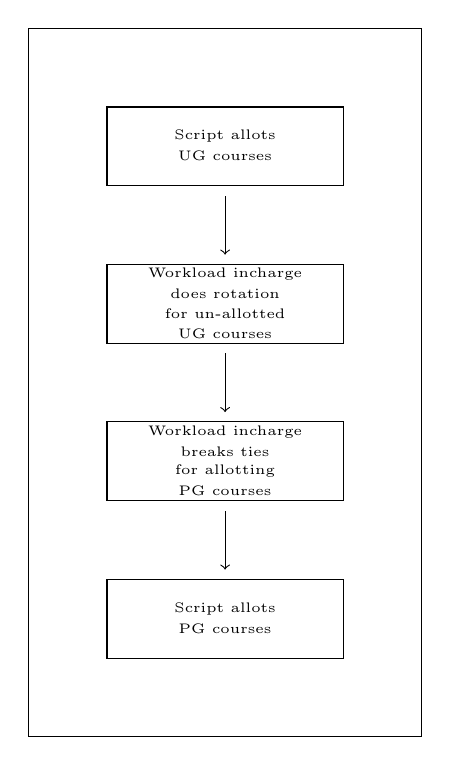
\begin{tikzpicture}
	\draw (-1,-1) rectangle (4,8);
	\draw (0,0) rectangle (3,1);
	\draw [<-] (1.5,1.125) -- (1.5,1.875);
	\draw (0,2) rectangle (3,3);
	\draw [<-] (1.5,3.125) -- (1.5,3.875);
	\draw (0,4) rectangle (3,5);
	\draw [<-] (1.5,5.125) -- (1.5,5.875);
	\draw (0,6) rectangle (3,7);
	\node at (1.5,6.625) {\tiny Script allots};
	\node at (1.5,6.375) {\tiny UG courses};
	\node at (1.5,4.875) {\tiny Workload incharge};
	\node at (1.5,4.625) {\tiny does rotation};
	\node at (1.5,4.375) {\tiny for un-allotted};
	\node at (1.5,4.125) {\tiny UG courses};
	\node at (1.5,2.875) {\tiny Workload incharge};
	\node at (1.5,2.625) {\tiny breaks ties};
	\node at (1.5,2.375) {\tiny for allotting};
	\node at (1.5,2.125) {\tiny PG courses};
	\node at (1.5,0.625) {\tiny Script allots};
	\node at (1.5,0.375) {\tiny PG courses};
\end{tikzpicture}
\end{document}